\chapter{Results} % Main chapter title
\noindent\textbf{\large Contents:}

\noindent\hrulefill
\noindent\startcontents[chapters]
\noindent\printcontents[chapters]{}{1}{}
\noindent\hrulefill
\label{Chapter4}

% \begin{itemize}
%     \item Cross-talk and detection region
%     \item analysis
%     \item conclusion and future work
% \end{itemize}

This chapter will go over the results of the simulation work as well as results from the optical testbed.

\section{Simulation Results}
\label{sec:sim}

With the control matrix in place, there needs to be data showing that there is a good linear correlation between the amplitude of the input wavefront aberration and what the system outputs.  Going through the process used in \S \ref{sec:RM}, a new set of aberrations were made with a range of amplitudes.   Then following the process described at the end of \S \ref{sec:CM}, we can compare the input amplitudes and what the code detects.  

\begin{figure}[H]
    \centering
    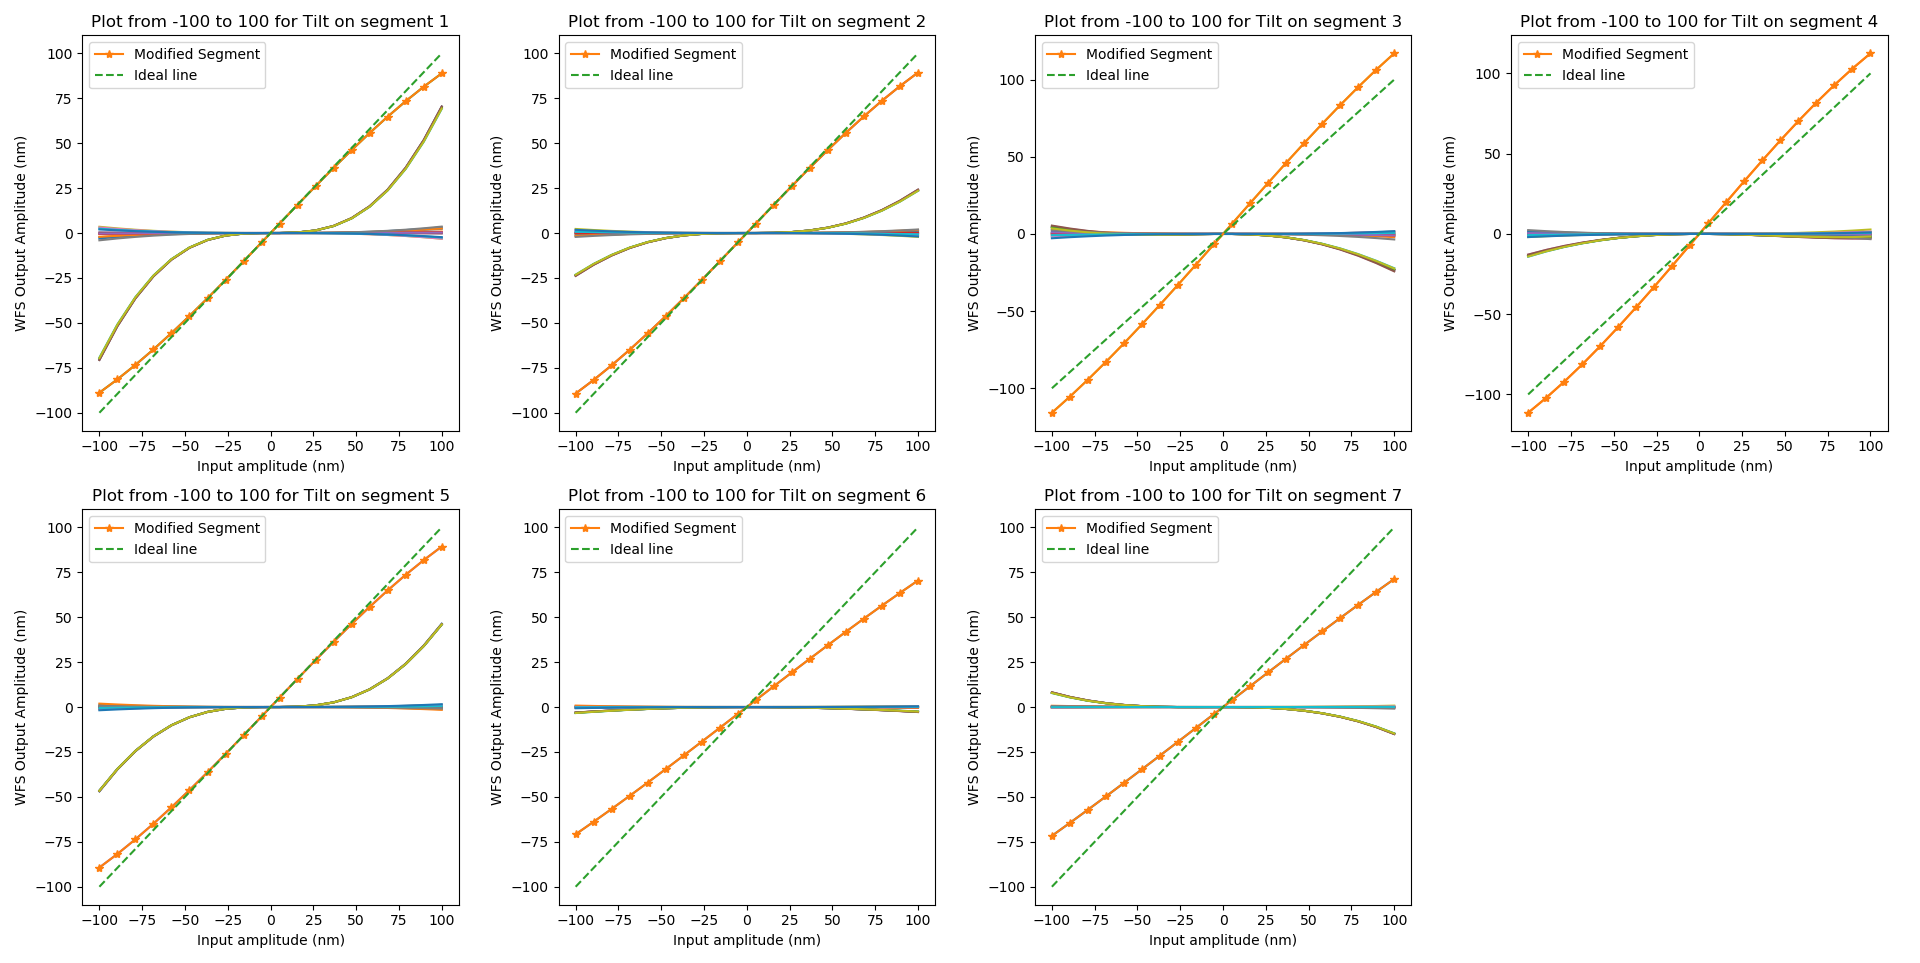
\includegraphics[width = 14cm]{Figures/Tilt_response100.png}
    \caption{Plots of each segments correlation between input aberration amplitudes and the output.  There are 21 lines for each mode in the modal basis set.}
    \label{fig:Tilt_100}
\end{figure}

As an example we will focus on the tilt of each segment.  As we can see in Figure \ref{fig:Tilt_100}, there is a linear region in the middle of each segment.  There is also some response from other modes.  This is cross-talk between other tilt modes from other segments.  However there is a region in the middle where cross-talk is limited.  Therefore the code ran again at to see the where the linear region lies.  In Figure \ref{fig:tilt30}, we can see there is limited cross-talk between the other modes and that there is a linear correlation between the input amplitude and the output amplitude.   

\begin{figure}[H]
    \centering
    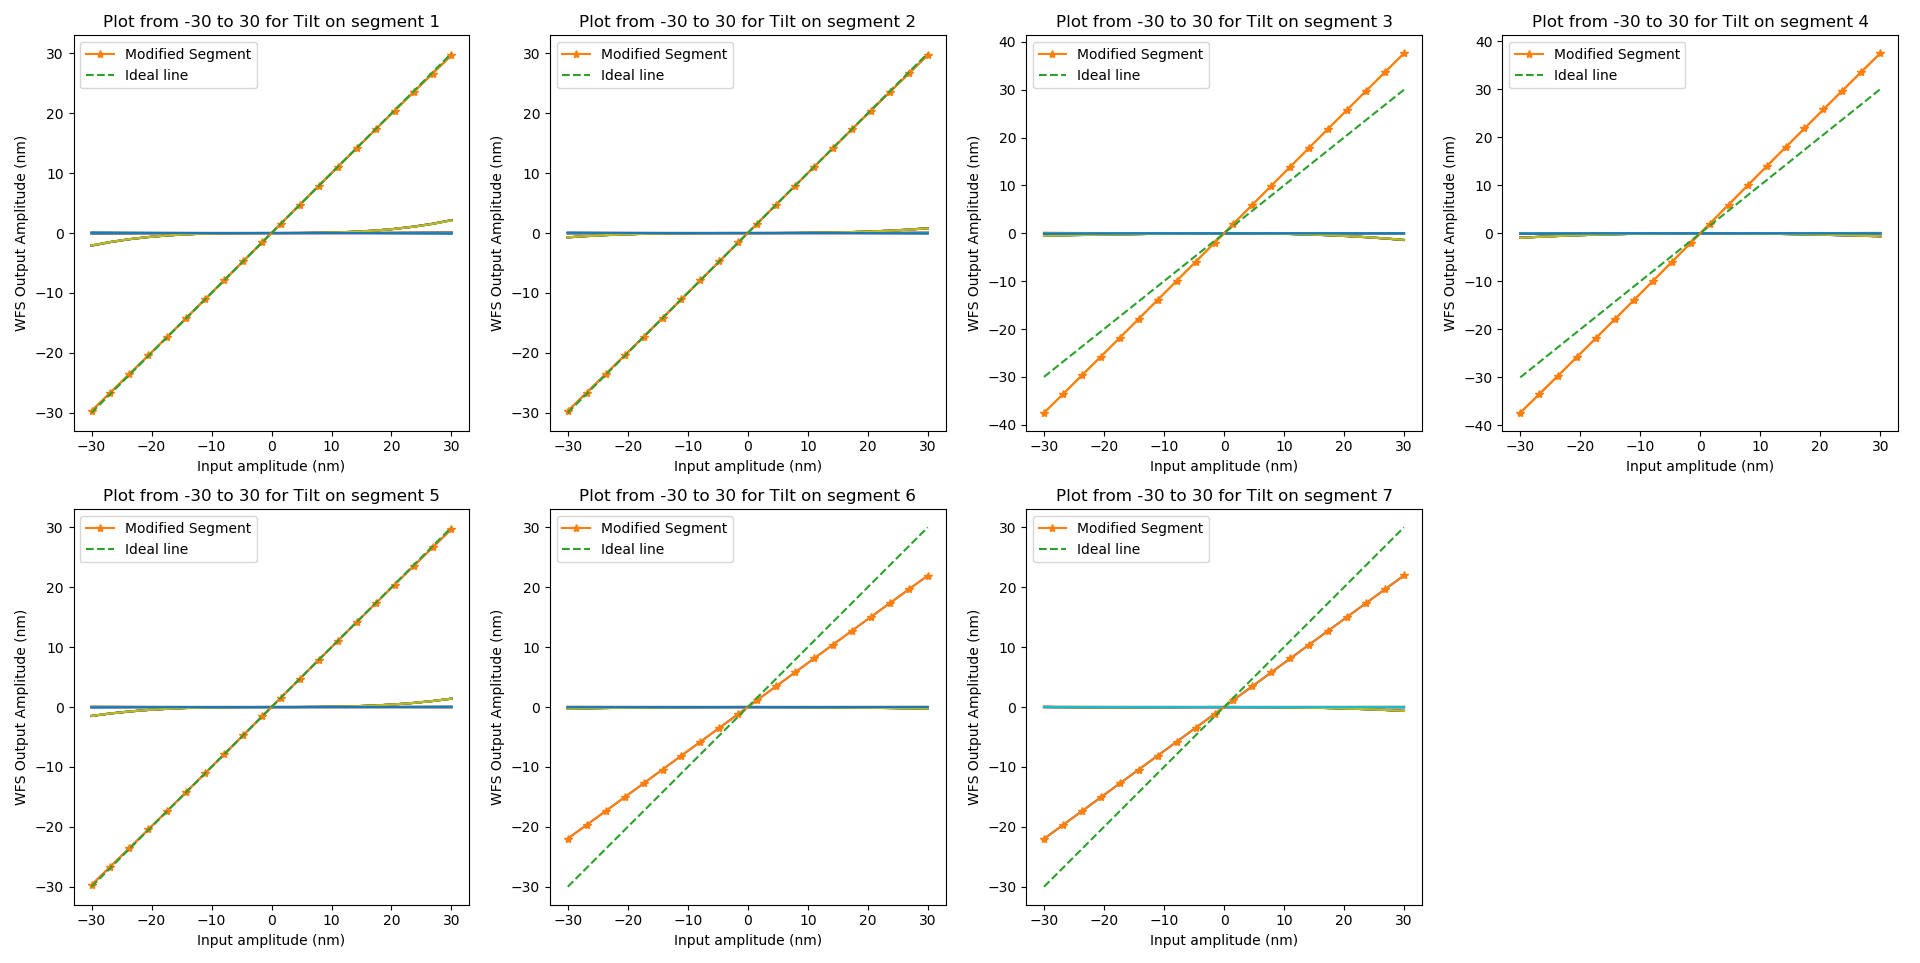
\includegraphics[width = 14cm]{Figures/Tilt_response30.png}
    \caption{Zoom in of Figure \ref{fig:Tilt_100} to show linear region in tilt response.}
    \label{fig:tilt30}
\end{figure}

It should be noted that there is a slope difference on segments on segments 3, 4, 6, and 7.  If we refer to Figure \ref{fig:amp_mask}, we can see that these segments are off axis and the aberration is perpendicular to the asymmetry.  This is purely hypothetical but could warrent further investigation.  However, these responses are still linear and can be corrected for.  This slope offset only occurs when tilt is applied.  All plots can be seen in Appendix \ref{AppendixB}

\section{Testbed Results}
\label{sec:testbed}

After putting the exposed images through the code, the out put is a wavefront error map and an output of each of the amplitudes of the modal basis set (Figure \ref{fig:wavefront_map}).  

\begin{figure}[H]
\centering
\begin{subfigure}{.5\textwidth}
  \centering
  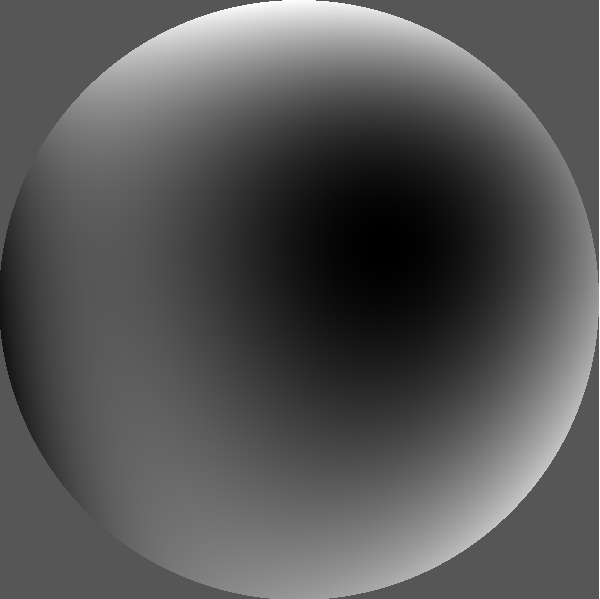
\includegraphics[width=6.5cm]{Figures/wavefront_error.png}
  \caption{A map of the sum total of the amplitudes for every mode in our modal basis set.}
  \label{fig:wavefront_map}
\end{subfigure}%
\begin{subfigure}{.5\textwidth}
  \centering
  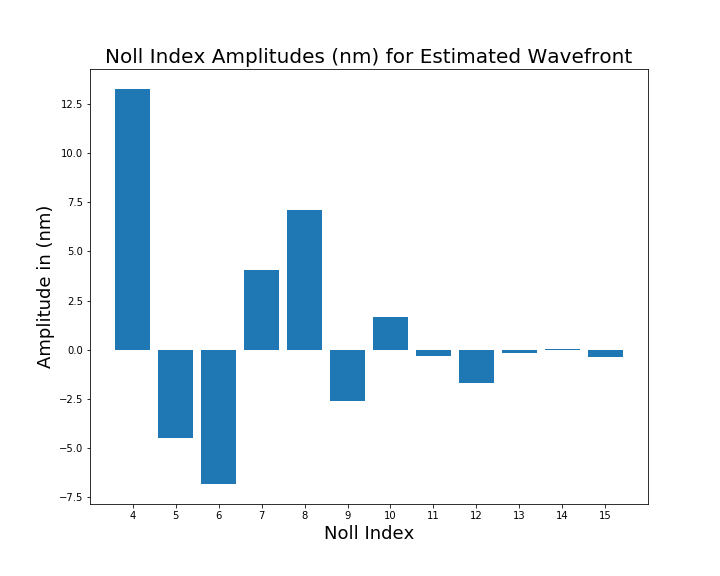
\includegraphics[width=8cm]{Figures/ampvnoll.png}
  \caption{The amplitude of each mode in nanometers}
  \label{fig:ampvsnoll}
\end{subfigure}
\caption{}
\label{fig:code_results}
\end{figure}


\section{Future Work}
\label{sec:future}